% !TEX root=/home/tavant/these/manuscript/src/manuscript.tex

\section{Full dielectric model }
  \label{sec-fulldiel}
  
  We have observed the effects of the electron emission and the electrostatic boundary condition separately in \cref{sec-diel_layer,sec-see}, respectively.
  
  \inlinenote{Anne: derniere phrase a mettre un peu plus loin}
  
  In \Cref{sec-see}, we observed three regimes depending on the emission rate.
  At high emissivity, the sheath is space-charge limited, resulting in an inverse sheath.
  At low emissivity, we obtain the standard sheath model with electron emission.
  The transition between the regimes passes by a oscillating regime.
  
  In \Cref{sec-diel_layer} we observed that when there is no emission, the dielectric boundary condition for the potential does not change the simulation results.
  In this section, we investigate the interaction between the two characteristics of the dielectric walls, especially with a high emission rate.
  More precisely, regime {\bf II} is the most interesting, as it features a complex behavior.
  Hence, we uses $\crover=45\,\volt$.
  
  \begin{figure}[hbtp]
    \centering
    \begin{tabular}{c c}
      \subfigure{see_diel_temporal}{a}{20,20} & 
      \subfigure{see_diel_space}{b}{20,20}
    \end{tabular}
    \caption{Comparison of the ({\bf a}) temporal and ({\bf b}) spatial evolution along the dielectric surface of the radial electric field at the wall calculated in PIC simulations compared to the electric field derived from the surface charge. }
    \label{fig-seediel_Er}
  \end{figure}
  \inlinenote{Anne: pas clairr le choix des echelles de temps..}
   
  \Cref{fig-seediel_Er} shows the ({\bf a}) temporal and ({\bf b}) spatial evolution along the dielectric surface of the radial electric field at the wall calculated in PIC simulations compared to the electric field derived from the surface charge, similarly  to \cref{fig-er_time}.{\bf b}.
  We can see that in contrast to the results of \cref{sec-diel_layer}, the two values are significantly different.
  The electric field measured in the \ac{PIC} simulation is rather uniform and constant, compared to the electric field at the surface calculated only based on the surface charge.
  Moreover, in \cref{fig-seediel_Er}.{\bf a}, we see that at around $t=2.1\,\second$, the electric field sign changes, meaning that the sheath passes from the \ac{SCL} regime {\bf I} to the normal regime {\bf III}, which is typical of regime {\bf II}.
  In contrast, the electric field derived from the surface charge does not shows this change of sheath regime.
  
  
  \begin{figure}[hbtp]
    \centering
    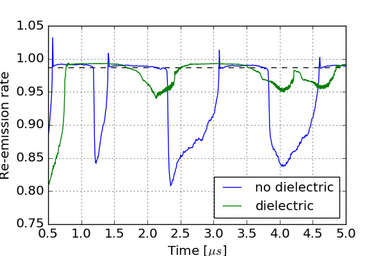
\includegraphics[width=\defaultwidth]{see_RSO}
    \caption{Temporal evolution of the mean electron emission rate $\ratepic$ for the same parameter $\crover=45\,\volt$, with and without the dielectric layer modeled.}
    \label{fig-rso_diel}
  \end{figure}
  
  \cref{fig-rso_diel} compares the temporal evolution of the mean electron emission rate $\ratepic$ for the same parameter $\crover=45\,\volt$, with and without the dielectric wall modeled.
  As previously, the dielectric width is $3\,\milli\meter$, and the electrodes are now $2.6\,\centi\meter$ apart (the geometry of the plasma domain is kept constant).
  We see that the oscillations occur for the two models.
  However, we can observe several differences.
  The first is the lower level of emission rate.
  When the walls are grounded, $\ratepic$ decreases at around $85\%$.
  Conversely, with the dielectric layer included, the emission rate does not decrease much below $95\%$.
  This results in a different overall mean emission rate, that can affect the particle and power balances, hence the mean electron temperature and the performance of the thruster.
  
  
  
  
  